\documentclass[11pt,aspectratio=169]{beamer}

% -------------------- THEME & LAYOUT --------------------
\usetheme{Madrid}
\usecolortheme{dolphin} % base color scheme
\usefonttheme{professionalfonts}
\setbeamercovered{transparent}
\setbeamertemplate{navigation symbols}{}   % remove navigation buttons
\setbeamertemplate{caption}[numbered]      % numbered captions
\setbeamertemplate{itemize items}[triangle]
\setbeamersize{text margin left=1.2cm,text margin right=1.2cm} % adjust to taste

% -------------------- GLOBAL FONT SETTINGS --------------------

% 1. Force the base beamer font to small
\setbeamerfont{normal text}{size=\small}

% 2. Force math environments to follow the "small" font size
\setbeamerfont{math text}{size=\small}
\setbeamerfont{equation}{size=\small}

% 3. Redefine \normalsize itself 
% This ensures equations and lists (which look for \normalsize) use  instead.
\let\oldnormalsize\normalsize
\renewcommand{\normalsize}{\oldnormalsize\small}

% 4. Ensure lists also stay small
\setbeamerfont{itemize/enumerate body}{size=\small}
\setbeamerfont{itemize/enumerate subbody}{size=\small}
% -------------------- FONTS & TYPOGRAPHY --------------------
\usepackage[T1]{fontenc}
\usepackage[utf8]{inputenc}
\usepackage{newpxtext,newpxmath} % Palatino-like font & math
\usepackage{microtype}

% -------------------- MATH, TABLES & GRAPHICS --------------------
\usepackage{amsmath,amssymb,amsfonts,mathtools}
\usepackage{bm,booktabs,siunitx,graphicx}
\graphicspath{{./}{./figures/}}
%for eps figures
\usepackage{graphicx}
\usepackage{epstopdf}
%for numbered equations
\setcounter{equation}{0}
\renewcommand{\theequation}{8.\arabic{equation}}

% -------------------- UTILITIES --------------------
\usepackage{appendixnumberbeamer}
\usepackage{ragged2e}
\usepackage{xspace}
\usepackage{csquotes}
\usepackage{xcolor}

% -------------------- HYPERREF --------------------
\hypersetup{
  colorlinks=false,
  pdfauthor={Francesca},
  pdftitle={Chapter 1 — The Value of Currency}
}

% -------------------- COLORS & EMPHASIS --------------------
\definecolor{myblue}{RGB}{0,70,140}
\definecolor{myred}{RGB}{180,30,30}
\definecolor{mygreen}{RGB}{0,120,70}
\definecolor{gold}{RGB}{184,134,11}

\setbeamercolor{title}{fg=gold}       % title page
\setbeamercolor{frametitle}{fg=gold}  % slide titles
\setbeamercolor{structure}{fg=gold}   % bullets, sections, links
\setbeamercolor{section in head/foot}{fg=gold,bg=black!10} % gold text on light background

% -------------------- FOOTLINE --------------------
\setbeamertemplate{footline}{
  \leavevmode%
  \hbox{%
    % Section links (hidden if no current section)
    \begin{beamercolorbox}[wd=0.7\paperwidth,ht=2.5ex,dp=1.5ex,leftskip=1.4em]{section in head/foot}%
      \ifx\insertsection\empty
        % nothing
      \else
        Section: \insertsection
      \fi
    \end{beamercolorbox}%
    % Frame number right
    \begin{beamercolorbox}[wd=0.3\paperwidth,ht=2.5ex,dp=1.5ex,leftskip=3.8cm]{section in head/foot}%
      \insertframenumber/\inserttotalframenumber
    \end{beamercolorbox}%
  }%
  \vskip1pt%
}

\newcommand{\highlight}[1]{\textcolor{myblue}{#1}}
\newcommand{\warning}[1]{\textcolor{myred}{#1}}

% -------------------- SHORTCUTS --------------------
\newcommand{\E}{\mathbb{E}}
\newcommand{\R}{\mathbb{R}}
\newcommand{\dd}{\mathrm{d}}
\newcommand{\mc}[1]{\mathcal{#1}}
\newcommand{\bb}[1]{\mathbb{#1}}
\newcommand{\uc}{U_c}
\newcommand{\zg}{Z_g}

% -------------------- TIGHTER DISPLAY MATH --------------------
\makeatletter
\g@addto@macro\normalsize{%
  \setlength\abovedisplayskip{8pt}%
  \setlength\belowdisplayskip{8pt}%
  \setlength\abovedisplayshortskip{6pt}%
  \setlength\belowdisplayshortskip{6pt}%
}
\makeatother
\setbeamertemplate{frametitle}{
  \nointerlineskip
  \begin{beamercolorbox}[wd=\paperwidth,ht=3.5ex,dp=1ex,center]{frametitle}
    \centering\insertframetitle
  \end{beamercolorbox}
}

% -------------------- METADATA --------------------
\title[Part II — Stabilization policies]{\textbf{Part II: Stabilization policies}\\[2pt]\large Chapter 8 — NK model with a banking sector}
\author{Pierpaolo Benigno}
\institute{}
\date{\today}

% -------------------- SECTION ROADMAP --------------------
\AtBeginSection[]
{
  \begin{frame}
    \tableofcontents[currentsection, hideothersubsections]
  \end{frame}
}

% -------------------- Bibliography --------------------
\usepackage[backend=biber,style=apa]{biblatex}
\addbibresource{sources.bib}

\begin{document}

% ===================== TITLE SLIDE =====================
\begin{frame}[plain] % 'plain' removes header/footer for the title slide

\begin{columns}[T,totalwidth=\textwidth]

% ----- Left column: Main title, professor, chapter -----
\begin{column}{0.45\textwidth}
\vspace{2cm}

% Main title
{\usebeamercolor[fg]{title}\LARGE\textbf{Monetary Economics}\\[0.3cm]
\LARGE\textbf{and Policy}} 

\vspace{0.5cm}

% Professor name and date
{\large\textit{Pierpaolo Benigno}}\\[0.1cm]

\vspace{1cm}

% Chapter and subtitle
{\usebeamercolor[fg]{frametitle}\large Chapter 8: New Keynesian Model with a Banking Sector}

\end{column}

% ----- Right column: Image -----
\begin{column}{0.55\textwidth}
\vspace{1cm}
\centering
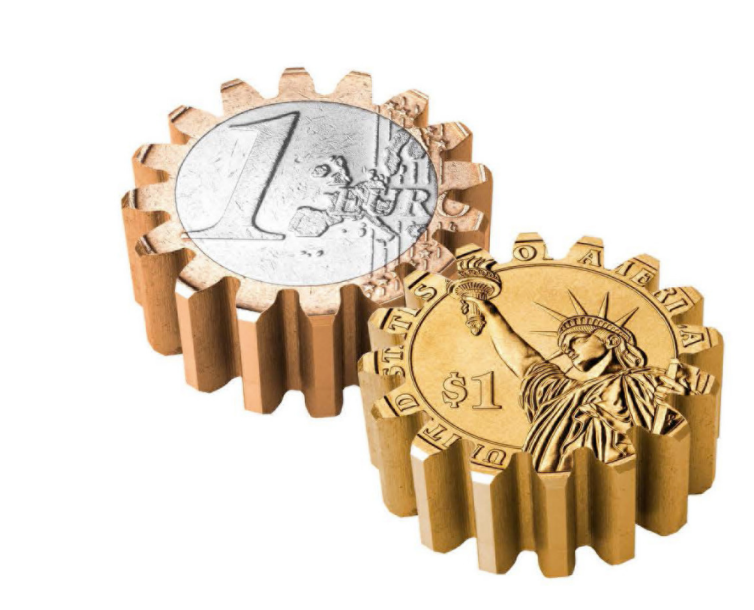
\includegraphics[width=0.9\linewidth]{Cover.png}
\end{column}

\end{columns}

% ----- Footer text (bottom-right corner) -----
\vspace*{2cm} % adjust if needed
\hfill{\large\textit{Prepared by Severin Rothen}}

\end{frame}


\begin{frame}{What We Will Learn}
\small
\begin{itemize}
  \item Why the benchmark New Keynesian model with a \textbf{single interest rate} misses key features of monetary transmission once banks and liquidity premia matter.
  \item How to introduce a \textbf{banking sector} where deposits provide \textbf{liquidity services} and government liabilities provide \textbf{collateral services}.
  \item How these frictions generate a \textbf{hierarchy of risk-free rates} (policy rate, deposit rate, credit-market rate) and a wedge between the policy rate and the rate relevant for consumption.
  \item How \textbf{government liquidity} (reserves and short-term public debt) affects aggregate demand by moving \textbf{liquidity premia}, beyond the standard interest-rate channel.
  \item How the model delivers a modified \textbf{log-linear aggregate demand equation} in which liquidity enters directly and the influence of expected future short rates is \textbf{attenuated}.
  \item How \textbf{optimal liquidity provision} (a Friedman-rule logic) calls for \textbf{satiating liquidity} when lump-sum taxes are available, and how this interacts with optimal stabilization policy.
\end{itemize}
\end{frame}


% OUTLINE
\begin{frame}{Outline}
\tableofcontents
\end{frame}


\section{Introduction}

%-----------------------------------------------------------
\begin{frame}{Limitations of the Standard NK Model}
  \begin{itemize}
    \item Benchmark New-Keynesian (NK) model:
    \begin{itemize}
      \item Single nominal interest rate $i_t$ for:
      \begin{itemize}
        \item Policy rate,
        \item Money-market rate,
        \item Credit-market rate relevant for households' Euler equation.
      \end{itemize}
      \item No explicit banking sector.
    \end{itemize}
    \medskip
    \item Great Financial Crisis 2007--2008:
    \begin{itemize}
      \item Large spreads between different credit standards, money-market rates, and the policy rate.
      \item Banks crucial for liquidity creation (deposits, reserves) and credit provision to households and firms.
    \end{itemize}
  \end{itemize}
\end{frame}

%-----------------------------------------------------------
\begin{frame}{Extended NK Model}
  \begin{itemize}
    \item We embed a banking sector into the NK framework.
    \medskip
    \item Two key financial frictions:
    \begin{itemize}

      \item \textbf{Households}: deposits $D_t$ provide liquidity services, they enter utility via $V(\frac{D_t}{P_t})$.
      \item \textbf{Banks}: government liabilities (reserves and treasury bills) provide collateral services for issuing deposits.
    \end{itemize}
    \medskip
    \item As a result, deposit rate $i_t^D$ carries a liquidity premium versus credit-market rate $i_t$. \item Reserves (and government debt) carry a liquidity premium versus deposit rate $i_t^D$.
    \end{itemize}
\end{frame}

%-----------------------------------------------------------
\begin{frame}{Key Results}
  \begin{itemize}
    \item Hierarchy of risk-free rates (in steady state and in equilibrium):
    $$i_t^X \;\le\; i_t^D \;\le\; i_t$$
    \item Transmission of monetary policy:
    \begin{itemize}
      \item Policy rate $i_t^X$ first affects banks' balance sheets, then affects deposit rate $i_t^D$ and credit-market rate $i_t$.
      \item Households' consumption/saving decisions depend on $i_t$, not directly on $i_t^X$.
    \end{itemize}
    \medskip
    \item Government liquidity:
    \begin{itemize}
      \item Total government liabilities $B_t^g$ (reserves + treasury bills) affect equilibrium liquidity premia, which changes the wedge between $i_t$ and $i_t^X$.
      \item Hence government liquidity directly influences aggregate demand and inflation.
    \end{itemize}
  \end{itemize}
\end{frame}

%-----------------------------------------------------------
\begin{frame}{Policy Implications}
  \begin{itemize}
    \item Central bank has two instruments:
    \begin{itemize}
      \item Policy rate on reserves $i_t^X$,
      \item Quantity of government liquidity $B_t^g$ (reserves + treasury bills).
    \end{itemize}
    \medskip
    \item Government liquidity affects:
    \begin{itemize}
      \item Liquidity premia on deposits and reserves,
      \item Credit-market rate $i_t$,
      \item Aggregate demand and inflation.
    \end{itemize}
    \medskip
    \item Important when central bank balance sheet expands/contracts:
    \begin{itemize}
      \item Quantitative easing / balance sheet policies,
      \item Exit from large balance sheets.
    \end{itemize}
  \end{itemize}
\end{frame}


%===========================================================
\section{Model}

%-----------------------------------------------------------
\begin{frame}{Banking Sector Balance Sheet}
  \begin{itemize}
    \item At time $t$, a representative bank has the balance sheet constraint:
\begin{align}
X_t + B_t^F + B_t = D_t + N_t.\label{8.1}
\end{align}
    \begin{itemize}
      \item $X_t$: Central bank reserves, with interest rate $i_t^X$.
      \item $B_t^F$: Treasury bills (government debt).
      \item $B_t$: Short-term private bonds, with interest rate $i_t$ (credit-market rate).
      \item $D_t$: Deposits, with interest rate $i_t^D$.
      \item $N_t$: Bank equity.
    \end{itemize}
    \medskip
    \item Treasury debt is fully backed by the central bank, therefore both pay interest rate $i_t^X$ and we define overall government debt as:
\begin{align*}
      B_t^g \equiv X_t + B_t^F.
\end{align*}
\end{itemize}
\end{frame}

    
% \item In equilibrium, only banks hold reserves; households use deposits for liquidity.


%-----------------------------------------------------------
\begin{frame}{Collateral and Zero Lower Bound}
  \begin{itemize}
    \item Intermediaries are subject to collateral requirement: 
$$ B_t^g \;\ge\; \rho D_t \;\ge\; 0,
      \qquad 0 \le \rho \le 1. $$
    \begin{itemize}
      \item When $\rho = 1$ we are in the case of narrow banking, i.e., all deposits must be fully backed by reserves.
      \item With $\rho = 0$ there is no collateral requirement.
    \end{itemize}
    \medskip
    \item Due to the possibility of converting reserves into cash there is a zero lower bound on reserves:
$$i_t^X \ge 0.$$
  \end{itemize}
\end{frame}

\begin{frame}{Short-term Private Bonds}
    \begin{itemize}
        \item In general $B_t$ can be positive (bank holds bonds) or negative (bank is borrowing). 
        \vspace{0.5cm}
        \item We will show later that $i_t \ge i_t^D$. This is because deposits provide liquidity services and, therefore, receive a liquidity premium whereas private bonds are risk-free but not liquid. 
    \end{itemize}
\end{frame}

%-----------------------------------------------------------
\begin{frame}{Bank Profits}
  \begin{itemize}
    \item Bank profits at time $t+1$ are:
\begin{align}
    \Psi_{t+1}^I
      = (1+i_t) B_t
        + (1+i_t^X) B_t^g
        - (1+i_t^D) D_t. \label{8.2}
\end{align}
    \item There is a limited liability constraint, i.e., profits must be non-negative in all states:
\begin{align}
    \Psi_{\min}^I
      = (1+i_t) B_t
        + (1+i_t^X) B_t^g
        - (1+i_t^D) D_t
      \;\ge\; 0.\label{8.3}
\end{align}
    \item Banks maximize expected rents:
\begin{align}
   \mathcal{R}_t
      = E_t\!\left[ \tilde{R}_{t,t+1}\,\Psi_{t+1}^I \right] - N_t,\label{8.4} 
\end{align}
    where $\tilde{R}_{t,t+1}$ is the stochastic nominal discount factor of households.
  \end{itemize}
\end{frame}

%-----------------------------------------------------------
\begin{frame}{Rents}
  \begin{itemize}
    \item Substitute profits \eqref{8.2} into expression \eqref{8.4}:
\begin{align*}
    \mathcal{R}_t
      = E_t\!\left[
        \tilde{R}_{t,t+1}\left(
          (1+i_t) B_t
          + (1+i_t^X) B_t^g
          - (1+i_t^D) D_t
        \right)\right] - N_t.
\end{align*}
\vspace{0.1cm}
\item Intermediaries choose $B_t, B_t^g, D_t, N_t$, with $B_t^g, D_t, N_t \ge 0$ to maximize \eqref{8.4} under budget constraint \eqref{8.1}, limited liability \eqref{8.3} and collateral constraint $B_t^g \ge \rho D_t$.
\vspace{0.3cm}
\item We will use here also the household's Euler condition that prices the market interest rate $i_t$ (discussed in details later):
$$E_t\{\tilde{R}_{t,t+1} (1+i_t)\} = 1.$$
  \end{itemize}
\end{frame}

%-----------------------------------------------------------
\begin{frame}{Obtaining the Rent Function}
  We start from \eqref{8.4}
$$\mathcal{R}_t
    = E_t\!\left[ \tilde{R}_{t,t+1}\,\Psi_{t+1}^I \right] - N_t.$$
  We use equation \eqref{8.1} inside profits $\Psi_{t+1}^I$ to obtain:
$$\Psi_{t+1}^I
    = (1+i_t)(D_t + N_t - B_t^g)
      + (1+i_t^X) B_t^g
      - (1+i_t^D) D_t.$$
  Rearranging:
$$\Psi_{t+1}^I
    = (1+i_t)N_t
      + \big[(1+i_t^X) - (1+i_t)\big] B_t^g
      + \big[(1+i_t) - (1+i_t^D)\big] D_t.$$
  Multiplying by $\tilde{R}_{t,t+1}$, taking expectations and using 
  $E_t\{\tilde{R}_{t,t+1} (1+i_t)\}=1$ yields: 
\begin{align}
    \mathcal{R}_t
    = \left[ \frac{1+i_t^X}{1+i_t} - 1\right] B_t^g
      - \left[ \frac{1+i_t^D}{1+i_t} - 1\right] D_t.\label{8.5}
\end{align}
\end{frame}

%-----------------------------------------------------------
\begin{frame}{Optimization Problem}
  \begin{itemize}
  \item Rent function \eqref{8.5} should be maximized under limited-liability constraint \eqref{8.3} and collateral constraint. 
\vspace{1em}
  \item Equity $N_t$ can always be raised to satisfy limited liability $\Rightarrow$ constraint not binding in optimum.
  \vspace{1em}
  \item There are different cases for supply of deposits: 
  \begin{itemize}
      \item Case 1: Excess Reserves $B_t^g > \rho D_t$
      \item Case 2: Binding collateral constraint $B_t^g = \rho D_t$ with special cases: 
      \begin{itemize}
          \item $\rho = 1$
          \item $\rho = 0$
      \end{itemize}
  \end{itemize}
  \end{itemize}
\end{frame}

%-----------------------------------------------------------
\begin{frame}{Case 1: Excess Reserves $B_t^g > \rho D_t$}
\small
  \begin{itemize}
    \item If collateral constraint is not binding, then $B_t^g$ and $D_t$ can be adjusted freely.
    \item If $\dfrac{1+i_t^X}{1+i_t} - 1 \neq 0$:
    \begin{itemize}
      \item Rents $\mathcal{R}_t$ can be made arbitrarily large by adjusting $B_t^g$.
      \item No equilibrium with finite rents.
    \end{itemize}
    \item Therefore in an equilibrium with finite holdings:
    $$\frac{1+i_t^X}{1+i_t} - 1 = 0
      \quad\Rightarrow\quad
      i_t^X = i_t.$$
    \item Given $i_t^X = i_t$, zero rents also require
$$\frac{1+i_t^D}{1+i_t} - 1 = 0
      \quad\Rightarrow\quad
      i_t^D = i_t^X = i_t.$$
    \item \textbf{Conclusion}: with excess reserves, all risk-free rates coincide.
  \end{itemize}
\end{frame}

%-----------------------------------------------------------
\begin{frame}{Case 2: Binding collateral ($B_t^g = \rho D_t$)}
  \begin{itemize}
    \item Substitute $B_t^g = \rho D_t$ into rent function \eqref{8.5}:
$$\mathcal{R}_t
      = \left[\frac{1+i_t^X}{1+i_t} - 1\right] \rho D_t
        - \left[\frac{1+i_t^D}{1+i_t} - 1\right] D_t.$$
        \vspace{0.3cm}
    \item Factor $D_t$:
$$\mathcal{R}_t
      = D_t \left\{
        \rho\left(\frac{1+i_t^X}{1+i_t} - 1\right)
        - \left(\frac{1+i_t^D}{1+i_t} - 1\right)
      \right\}.$$
\end{itemize}
\end{frame}






%-----------------------------------------------------------
\begin{frame}{Deposit Rate}
\begin{itemize}
    \item Zero-rent condition ($\mathcal{R}_t=0$ and $D_t>0$) implies:
$$\rho\left(\frac{1+i_t^X}{1+i_t} - 1\right)
      = \left(\frac{1+i_t^D}{1+i_t} - 1\right).$$
      \vspace{0.3cm}
     \item Rearranging:
\begin{align}
    1+i_t^D
    = \rho(1+i_t^X) + (1-\rho)(1+i_t).\label{8.6}
\end{align}
    \item When rents are zero, the deposit rate is a weighted average of policy rate and credit-market rate.
\end{itemize}

\end{frame}

%-----------------------------------------------------------
\begin{frame}{Special Cases: $\rho = 1$ and $\rho = 0$}
  \begin{itemize}
    \item \textbf{Narrow banking} ($\rho = 1$):
    \begin{itemize}
        \item Using \eqref{8.6} and $\rho=1$ it follows that 
        $$1+i_t^D = 1+i_t^X
      \quad\Rightarrow\quad
      i_t^D = i_t^X.$$
        \item Generally $i_t \ge i_t^D = i_t^X$.
    \end{itemize}
\medskip
    \item \textbf{No collateral requirement} ($\rho = 0$):
    \begin{itemize}
        \item Equation \eqref{8.6} and $\rho=0$ yields: 
    $$1+i_t^D = 1+i_t
      \quad\Rightarrow\quad
      i_t^D = i_t.$$
    \item When reserves are supplied at a positive level it must be that $i_t = i_t^X$. 
    \item Therefore all risk-free rates coincide:
    $$i_t = i_t^D = i_t^X.$$
    \end{itemize}
  \end{itemize}
\end{frame}

\begin{frame}{Benchmark New-Keynesian Model as a special case}

    \begin{itemize}
        \item The standard New-Keynesian model with a \textbf{single} nominal interest rate
        (policy rate = deposit rate = credit-market rate) is nested in this framework when
        either of the following holds:
        \begin{enumerate}
            \item \textbf{Excess government liquidity:} the collateral constraint is slack,
            \[
                B_t^g > \rho D_t,
            \]
            so banks hold reserves in excess of what is required.
            \item \textbf{No collateral requirement / no liquidity services from $B_t^g$:}
            \[
                \rho = 0.
            \]
        \end{enumerate}
        \item In both cases, all risk-free rates are equalized:
        \[
            i_t^X = i_t^D = i_t.
        \]
    \end{itemize}
\end{frame}


\begin{frame}{Equity Demand}
  \begin{itemize}
    \item Substituting the balance sheet \eqref{8.1} into the limited-liability constraint \eqref{8.3}:
    \[
      (1+i_t)(D_t + N_t - B_t^g)
      + (1+i_t^X)B_t^g
      - (1+i_t^D)D_t \ge 0.
    \]
    \item Rearranging for $N_t$:
    \[
      N_t \ge \frac{i_t^D - i_t}{1+i_t}D_t
             + \frac{i_t - i_t^X}{1+i_t}B_t^g.
    \]
    \item Using the expressions for the deposit rate and the collateral constraint, this implies
    \[
      N_t \ge 0.
    \]
    \item Since all assets are riskless, equity is non-negative and can be zero in equilibrium.
  \end{itemize}
\end{frame}


%-----------------------------------------------------------
\begin{frame}{Household Preferences}
  \begin{itemize}
    \item Representative household maximizes:
    \begin{align}
        E_{t_0}\left\{
        \sum_{t=t_0}^\infty
          \beta^{t-t_0} \xi_t
          \left[
            U(C_t)
            + V\!\left(\frac{D_t}{P_t}\right)
            - \int_0^1 \frac{L_t(j)^{1+\eta}}{1+\eta} \, dj
          \right]
      \right\}. \label{8.7}
    \end{align}
    \begin{itemize}
      \item $U(\cdot)$: concave, differentiable utility from consumption $C_t$ (Dixit-Stiglitz aggregator).
      \item $V(\cdot)$: concave, differentiable utility from real deposits $D_t/P_t$.
      \item $V_d(\cdot)=0$ for $D_t/P_t \ge \bar{d}$ (satiation level $\bar{d}$).
      \item $\xi_t$: preference shock.
      \item $\eta \ge 0$: inverse of the Frisch elasticity of labor.
    \end{itemize}
    \item The only difference to benchmark NK model is that households get utility from deposits, through liquidity term $V(\cdot)$.
  \end{itemize}
\end{frame}

%-----------------------------------------------------------
\begin{frame}{Household Budget Constraint}
  \begin{itemize}
    \item Flow budget constraint:
\begin{align*}
    P_t C_t + D_t + (1+i_{t-1}) B_{t-1} + N_t + T_t
      \;\le\; (1+i_{t-1}^D) D_{t-1} + B_t
        + \int_0^1 W_t(j) L_t(j) dj \\
        + \Psi_t^I + \Psi_t.
\end{align*}
      \item LHS: consumption, new deposits, repayment of bonds, new equity, taxes.
      \item RHS: deposit returns, new bonds, labor income, profits from intermediaries ($\Psi_t^I$) and firms ($\Psi_t$).
    \item Households trade:
    \begin{itemize}
      \item Illiquid, risk-free bonds $B_t$ at rate $i_t$ ($B_t>0$ denotes debt),
      \item Deposits $D_t$ at rate $i_t^D$, providing liquidity services,
      \item Equity $N_t$ for banks.
    \end{itemize}
    \item The consumption/saving choices are subject to an appropriate borrowing limit.
  \end{itemize}
\end{frame}

%-----------------------------------------------------------
\begin{frame}{Euler Equation for Illiquid Bonds}
  \begin{itemize}
    \item Optimal choice of $B_t$ implies the condition:
    \begin{align}
        E_t\{\tilde{R}_{t,t+1}\} = \frac{1}{1+i_t}, \label{8.8}
    \end{align}
    where the nominal stochastic discount factor is: $$\tilde{R}_{t,t+1}
      = \beta
        \frac{\xi_{t+1} U_c(C_{t+1})}{\xi_t U_c(C_t)}
        \frac{P_t}{P_{t+1}}.$$
    \item This is the standard NK asset-pricing condition: $$1 = E_t\left[
      \tilde{R}_{t,t+1} (1+i_t)
      \right].$$
    \item $i_t$ is the \emph{credit-market nominal interest rate} relevant for consumption-savings.
  \end{itemize}
\end{frame}

%-----------------------------------------------------------
\begin{frame}{FOC for Deposits}
  \begin{itemize}
    \item FOC for deposits $D_t$:
    \begin{align}
        1
      = \varrho_t
        + (1+i_t^D) E_t\{\tilde{R}_{t,t+1}\}, \label{8.9}
    \end{align}
    where $\varrho_t$ is the liquidity premium: $$\varrho_t
      = \frac{V_d(\frac{D_t}{P_t})}{U_c(C_t)}.$$
    \item Combining \eqref{8.8} with \eqref{8.9}
    we obtain:
    \begin{align}
        1+i_t^D = (1-\varrho_t)(1+i_t). \label{8.9.5}
    \end{align}
  \end{itemize}
\end{frame}

%-----------------------------------------------------------
\begin{frame}{Liquidity Satiation and Equity}
  \begin{itemize}
    \item With $0 \le \varrho_t < 1$:
    \begin{itemize}
      \item Deposits pay a lower interest rate than illiquid bonds:
      $$i_t^D \le i_t.$$
      \item The wedge $i_t - i_t^D$ is determined by liquidity services.
    \end{itemize}
    \item If the economy is satiated with liquidity, i.e., $\varrho_t = 0$ then the two rates coincide ($i_t^D = i_t)$
    \item FOC for equity:
    $$N_t = E_t\{\tilde{R}_{t,t+1} \Psi_{t+1}^I\}.$$
    \item Finally, the intertemporal budget constraint of the consumer holds with equality at all times.
  \end{itemize}
\end{frame}


%-----------------------------------------------------------
\begin{frame}{Firms: Technology and Pricing}
  \begin{itemize}
    \item Continuum of firms $j \in [0,1]$ produce $Y_t(j) = A_t L_t(j),$ with labor productivity $A_t$.
    \item Demand for variety $j$ is $Y_t(j)
      = \left(\frac{P_t(j)}{P_t}\right)^{-\theta} Y_t,$ with elasticity of substitution $\theta>1$.
    \item The aggregate price index $P_t$ is the Dixit--Stiglitz aggregator.
    \item Calvo price setting:
    \begin{itemize}
      \item Fraction $1-\alpha$ can reset prices each period.
      \item Non-adjusting firms index prices to target inflation $\Pi$.
    \end{itemize}
  \end{itemize}
\end{frame}

%-----------------------------------------------------------
\begin{frame}{AS Block}
  \begin{itemize}
    \item As in the benchmark NK model of Chapter 5 (with the only difference that here $G_t=0$), equilibrium pricing conditions yield:
    $$\left(
        \frac{1-\alpha(\Pi_t/\Pi)^{\theta-1}}
             {1-\alpha}
      \right)^{\frac{1+\theta\eta}{\theta-1}}
      = \frac{F_t}{J_t},$$
    with
    $$ F_t
      = \xi_t U_c(Y_t)\frac{Y_t}{\mu_t}
        + \alpha\beta\,E_t\left\{
           \left(\frac{\Pi_{t+1}}{\Pi}\right)^{\theta-1} F_{t+1}
        \right\},$$
$$  J_t
      = \xi_t\left(\frac{Y_t}{A_t}\right)^{1+\eta}
        + \alpha\beta\,E_t\left\{
           \left(\frac{\Pi_{t+1}}{\Pi}\right)^{\theta(1+\eta)} J_{t+1}
        \right\}.$$
  \end{itemize}
\end{frame}


%-----------------------------------------------------------
\begin{frame}{Government}
  \begin{itemize}
    \item Consolidate treasury and central bank.
    \item Flow budget constraint:
    \begin{align}
        B_t^g
      = (1+i_{t-1}^X) B_{t-1}^g
        + \tau_t^s P_t Y_t
        - T_t, \label{8.10}
    \end{align}
    where
    \begin{itemize}
      \item $B_t^g$: total government liabilities (including reserves),
      \item $\tau_t^s$: subsidy to firm revenues (markup correction),
      \item $T_t$: lump-sum taxes.
    \end{itemize}
    \medskip
    \item Central bank fully backs treasury, therefore overall government debt is not subject to a solvency condition. 
  \end{itemize}
\end{frame}

%===========================================================
\section{Equilibrium}

%-----------------------------------------------------------

\begin{frame}{Equilibria in Assets and Goods Markets}
    \begin{itemize}
        \item Asset-market equilibrium: 
        \begin{itemize}
            \item All government bonds $B^g$ held by intermediaries.\item Deposits $D$ are held by the households. 
            \item $B$ issued by the households is an asset for the intermediaries.
        \end{itemize}
        \vspace{0.3cm}
        \item Goods market equilibrium implies $Y_t = C_t$ for each $t \ge t_0.$
    \end{itemize}
\end{frame}

\begin{frame}{AD Block}
  \begin{itemize}
    \item Recall the relationship between the deposit-, policy- and credit-market rate \eqref{8.6} (binding collateral):
    \begin{align}
    1+i_t^D
      = \rho(1+i_t^X) + (1-\rho)(1+i_t). \label{8.11}
    \end{align}
    \item From \eqref{8.9.5}, the spread between the deposit rate and credit-market rate must satisfy 
    \begin{align}
         \frac{1+i_t^D}{1+i_t}
      = 1 - \frac{V_d(D_t/P_t)}{U_c(Y_t)}, \label{8.12}
    \end{align} where, using the definition of the stochastic discount factor, \eqref{8.8} implies: 
    \begin{align}
          \frac{1}{1+i_t}
      = E_t\left\{
         \beta\frac{\xi_{t+1}U_c(Y_{t+1})}{\xi_t U_c(Y_t)}\frac{P_t}{P_{t+1}}
        \right\}. \label{8.13}
    \end{align}
  \end{itemize}
\end{frame}

%-----------------------------------------------------------
\begin{frame}{AS Block}
  \begin{itemize}
    \item As already stated, the AS block of the model is as in Chapter 5: 
    \begin{align}
        \left(
        \frac{1-\alpha(\Pi_t/\Pi)^{\theta-1}}
             {1-\alpha}
      \right)^{\frac{1+\theta\eta}{\theta-1}}
      = \frac{F_t}{J_t}, \label{8.14}
    \end{align}
    with
    \begin{align}
        F_t
      &= \xi_t U_c(Y_t)\frac{Y_t}{\mu_t}
        + \alpha\beta\,E_t\left\{
           \left(\frac{\Pi_{t+1}}{\Pi}\right)^{\theta-1} F_{t+1}
        \right\}, \label{8.15} \\
        J_t
      &= \xi_t\left(\frac{Y_t}{A_t}\right)^{1+\eta}
        + \alpha\beta\,E_t\left\{
           \left(\frac{\Pi_{t+1}}{\Pi}\right)^{\theta(1+\eta)} J_{t+1}
        \right\}, \label{8.16}
    \end{align} and markup $\mu_t = \frac{\theta}{(\theta -1)(1 + \tau_t^s)}$ where $\tau_t^s$ is the tax/subsidy. 
  \end{itemize}
\end{frame}

\begin{frame}{Constraints}
    \begin{itemize}
        \item Government flow budget constraint \eqref{8.11}: 
        \begin{align}
            B_t^g
      = (1+i_{t-1}^X) B_{t-1}^g
        + \tau_t^s P_t Y_t
        - T_t. \label{8.17}
        \end{align}
        \item Intertemporal resource constraint: 
        \begin{align}
            \frac{(1+i_{t-1}^X)B_{t-1}^g}{P_t}
      = E_t\left\{
        \sum_{T=t}^\infty
        \beta^{T-t}\frac{\xi_T U_c(Y_T)}{\xi_t U_c(Y_t)}
        \left[
          \frac{T_T}{P_T}
          - \tau_T^s Y_T
          + \frac{i_T - i_T^X}{1+i_T}\frac{B_T^g}{P_T}
        \right]
      \right\}. \label{8.18}
        \end{align}
        \item Collateral constraint:
        \begin{align}
            B_t^g \ge \rho D_t. \label{8.19}
        \end{align}
    \end{itemize}
\end{frame}

%-----------------------------------------------------------
\begin{frame}{Equilibrium and Policy Regime}
\begin{itemize}
  \item An equilibrium is a \textbf{set of stochastic processes}
  \[
    \{ P_t,\, i_t,\, i_t^D,\, i_t^X,\, Y_t,\, F_t,\, J_t,\, D_t,\, T_t,\, B_t^g \}_{t=t_0}^{\infty},
  \]
  satisfying:
  \begin{itemize}
    \item Equations \eqref{8.11}--\eqref{8.17}, \eqref{8.19}, for each $t \ge t_0$ and \eqref{8.18} considering
    \item Inflation definition $\Pi_t \equiv P_t/P_{t-1}$,
    \item Inequality constraint $i_t \ge i_t^X \ge 0$,
    \item Given exogenous processes $\{\xi_t, A_t, \tau_t^s\}_{t=t_0}^{\infty}$ and initial conditions.
  \end{itemize}
  \medskip
  \item \textbf{Policy degrees of freedom}:
  \begin{itemize}
    \item Central bank sets the interest rate on reserves $\{i_t^X\}_{t=t_0}^{\infty}$,
    \item Central bank and treasury jointly set total government liabilities
    $\{B_t^g\}_{t=t_0}^{\infty}$ (including reserves).
  \end{itemize}
\end{itemize}
\end{frame}

%-----------------------------------------------------------
\begin{frame}{Relation to the Benchmark NK Model}
\begin{itemize}
  \item Key departure from the benchmark NK model (Chapter~5):
  \begin{itemize}
    \item \textbf{Government debt} directly influences aggregate demand,
    \item Transmission occurs through equations \eqref{8.12} and \eqref{8.19}.
  \end{itemize}
\vspace{0.4cm}
\item The standard NK model is \textbf{nested} as a special case:
  \begin{itemize}
    \item When liquidity is fully satiated:
    \[
      V_d(\cdot) = 0.
    \]
  \end{itemize}
\end{itemize}
\end{frame}


%===================================================%===========================================================
\section{Log-linear approximation}
%===========================================================

%-----------------------------------------------------------
\begin{frame}{Log-linearization: Notation and Focus}
\begin{itemize}
  \item Log-deviation (unless otherwise noted): $\hat X_t \equiv \ln(X_t/X)$.
  \item Inflation: $\Pi_t \equiv P_t/P_{t-1}$,\quad $\pi_t \equiv \ln \Pi_t$,\quad target $\pi \equiv \ln\Pi$.
  \item Real deposits: $d_t \equiv D_t/P_t$,\quad $\hat d_t \equiv \ln(d_t/d)$.
  \item Interest-rate deviations:
  \[
    \hat\imath_t \equiv \ln\!\Big(\tfrac{1+i_t}{1+i}\Big),\quad
    \hat\imath_t^X \equiv \ln\!\Big(\tfrac{1+i_t^X}{1+i^X}\Big),\quad
    \hat\imath_t^D \equiv \ln\!\Big(\tfrac{1+i_t^D}{1+i^D}\Big).
  \]
  \item Goal: express the NK system in log-linear form, highlighting the role of
  \textbf{(i) multiple rates} and \textbf{(ii) liquidity (deposits)}.
\end{itemize}
\end{frame}

%-----------------------------------------------------------
\begin{frame}{New-Keynesian Phillips curve}
\begin{itemize}
  \item Log-linear AS equation (NKPC):
  \begin{align}
    \pi_t - \pi
    = \kappa(\hat Y_t - \hat Y_t^n)
    + \beta E_t(\pi_{t+1}-\pi). \label{8.20}
  \end{align}
  \item Natural output:
  \[
    \hat Y_t^n
    = \frac{1+\eta}{\sigma^{-1}+\eta}\hat A_t
      -\frac{1}{\sigma^{-1}+\eta}\hat\mu_t,
    \qquad
    \sigma \equiv -\frac{U_{cc}Y}{U_c}>0.
  \]
  \item Benchmark NK AS equation holds.
\end{itemize}
\end{frame}

%-----------------------------------------------------------
\begin{frame}{AD in Terms of the Credit-Market Rate}
\begin{itemize}
  \item Log-linearizing the Euler equation \eqref{8.13}:
  \begin{align}
    \hat Y_t
    = E_t\hat Y_{t+1}
      - \sigma\Big(\hat\imath_t
      - E_t(\pi_{t+1}-\pi)
      + E_t\Delta\hat\xi_{t+1}\Big). \label{8.21}
  \end{align}
  \item Preference growth term: $\Delta\hat\xi_{t+1}\equiv \hat\xi_{t+1}-\hat\xi_t$.
  \item Key difference vs benchmark NK: \eqref{8.21} depends on the \textbf{credit-market rate} $i_t$ (not directly the policy rate).
\end{itemize}
\end{frame}

%-----------------------------------------------------------
\begin{frame}[label=Rate Mapping]{Money Market Rates}
\begin{itemize}
  \item Banking sector implies the following (log-linear) relationship:
  \begin{align}
    \hat\imath_t
    = \hat\imath_t^X
      + \frac{1-\nu}{\rho-\nu}\big(\hat\imath_t-\hat\imath_t^D\big),
    \label{8.22}
  \end{align}
  where $\nu \equiv V_d/U_c$ (evaluated at steady state) and $\nu<\rho$.
  \item Interpretation:
  \begin{itemize}
    \item The policy rate $i_t^X$ transmits to the economy through bank pricing of deposits.
    \item The spread $(\hat\imath_t-\hat\imath_t^D)$ matters for the mapping from policy to the credit rate.
  \end{itemize}
\end{itemize}
\vspace{0.1cm}
\begin{center}
\hyperlink{Appendix H}{\beamerbutton{Derivation of Money Market Rates and Deposit Demand (Appendix)}}
\end{center}
\end{frame}

%-----------------------------------------------------------
\begin{frame}{Liquidity Demand}
\begin{itemize}
  \item Liquidity market equilibrium implies:
  \begin{align}
    \hat d_t
    = d_y \hat Y_t
      - d_i\big(\hat\imath_t-\hat\imath_t^D\big),
    \label{8.23}
  \end{align}
  where
  \[
    d_y \equiv \frac{\sigma_d}{\sigma},\qquad
    d_i \equiv \sigma_d\frac{1-\nu}{\nu},\qquad
    \sigma_d \equiv -\frac{V_d}{V_{dd}d}.
  \]
  \item Higher output raises liquidity demand; a higher spread $(i_t-i_t^D)$ lowers liquidity demand.
\end{itemize}
\end{frame}

%-----------------------------------------------------------
\begin{frame}{Benchmark NK as a Special Case (Full Satiation)}
\begin{itemize}
  \item If liquidity is fully satiated: $\nu=0$.
  \vspace{1em}
  \item Then rates equalize in and out of steady state:
  \[
    i_t^D = i_t^X = i_t.
  \]
\vspace{1em}
  \item AD collapses to the benchmark NK AD curve:
  \begin{align}
    \hat Y_t
    = E_t\hat Y_{t+1}
      - \sigma\Big(\hat\imath_t^X
      - E_t(\pi_{t+1}-\pi)
      + E_t\Delta\hat\xi_{t+1}\Big).
    \label{8.24}
  \end{align}
\end{itemize}
\end{frame}

%-----------------------------------------------------------
\begin{frame}{Aggregate Demand with Liquidity}
\begin{itemize}
  \item In the general case ($\nu>0$), combining \eqref{8.21}, \eqref{8.22}, \eqref{8.23} yields:
  \begin{align}
    \hat Y_t
    &= \nu_\rho E_t \hat Y_{t+1}
     - \sigma\nu_\rho\Big(\hat\imath_t^X
      - E_t(\pi_{t+1}-\pi)
      + E_t\Delta\hat\xi_{t+1}\Big)
     + d_y^{-1}(1-\nu_\rho)\hat d_t,
     \label{8.25}
  \end{align}
  where
  \[
    \nu_\rho \equiv 1-\rho^{-1}\nu \in (0,1).
  \]
\end{itemize}
\end{frame}

%-----------------------------------------------------------
\begin{frame}{Main Implications vs the Benchmark NK Model}
\begin{itemize}
  \item \textbf{Liquidity shifts AD directly:} deposits $\hat d_t$ enter \eqref{8.25}.
  \vspace{1em}
  \item \textbf{Attenuated forward guidance:} $\nu_\rho<1$ reduces the effect of expected future output (and thus expected future policy) on current output.
  \vspace{1em}
  \item \textbf{Two transmission margins:}
  \begin{itemize}
    \item Policy rate $i_t^X$ affects demand through the banking-sector wedge \eqref{8.22},
    \item Liquidity $d_t$ affects demand directly \eqref{8.25}.
  \end{itemize}
  \vspace{1em}
  \item Higher deposits ---corresponding to a larger supply of government liquidity--- are \textbf{expansionary} for output.
\end{itemize}
\end{frame}

%-----------------------------------------------------------

%===========================================================
\section{Impulse Responses}


%---------------------------------------------------
\begin{frame}{Impulse Response to a Policy-Rate Shock}

\begin{columns}[T]
\small
% -------- Left column: figure --------
\begin{column}{0.5\textwidth}
\begin{figure}
\centering
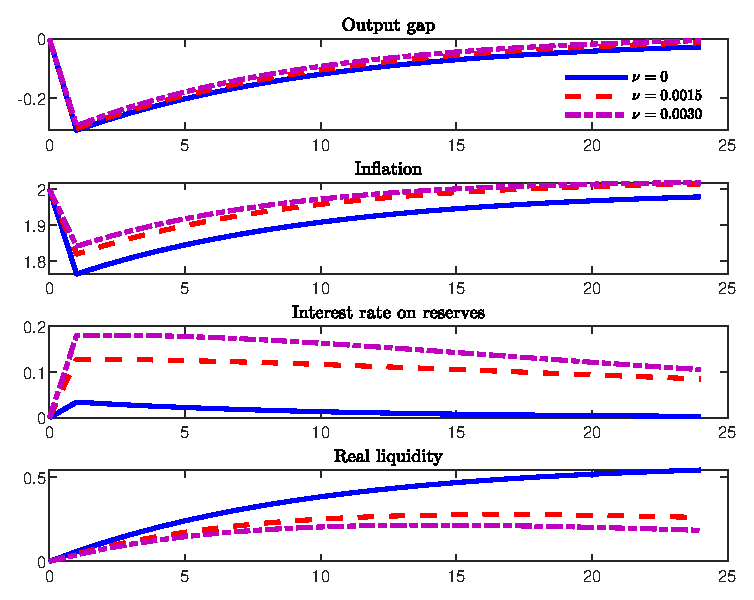
\includegraphics[width=\linewidth]{Figure12}
\caption{Impulse Response to a Shock to the Interest Rate on Reserves}
\label{Figure8.1}
\end{figure}
\end{column}

% -------- Right column: description --------
\begin{column}{0.5\textwidth}
\small
\begin{itemize}
  \item Monetary policy follows the interest-rate rule 
  $\hat{\imath}_t^{X}
= \phi_{\pi}\,(\pi_t - \pi)
  + \phi_{y}\,\hat{Y}_t
  + e_t$ 
  
  with $e_t = \rho_e e_{t-1} + \varepsilon_{1,t}$ and $0 \le \rho_e \le 1$ as well as $\phi_\pi, \phi_y \ge 0$.
  \vspace{1em}
  \item The Figure shows the responses of output gap, inflation, interest rate on reserves, real liquidity to a one-time shock $\varepsilon_{1,t}$.
  
\end{itemize}
\end{column}
\end{columns}
\end{frame}

\begin{frame}{Impulse Response to a Policy Shock}
\small
    \begin{itemize}
        \item The figure shows the impulse responses for three different calibrations of $\nu \in \{0,\,0.0015,\,0.003\}$ which implies interest rate spreads of $ (i - i^D) \in \{0,\,60,\,120\}$ in basis points at annual rates. 
        
  \item When $\nu = 0$, the benchmark NK model is nested:
  \begin{itemize}
    \item A positive interest-rate shock is contractionary, lowering output gap and inflation.
    \item Liquidity does not affect aggregate demand; real liquidity rises only mechanically as inflation falls.
  \end{itemize}

  \item When $\nu > 0$, liquidity influences aggregate demand:
  \begin{itemize}
    \item Higher real liquidity mitigates the decline in the output gap and inflation.
    \item The stabilizing effect is present but quantitatively small.
  \end{itemize}

  \item Because inflation falls less when $\nu > 0$, real liquidity increases by less than in the $\nu = 0$ case.
\end{itemize}


\end{frame}


%-----------------------------------------------------------

\begin{frame}{Impulse Response to a Liquidity Shock}

\begin{columns}[T]
\small
% -------- Left column: figure --------
\begin{column}{0.5\textwidth}
\begin{figure}
\centering
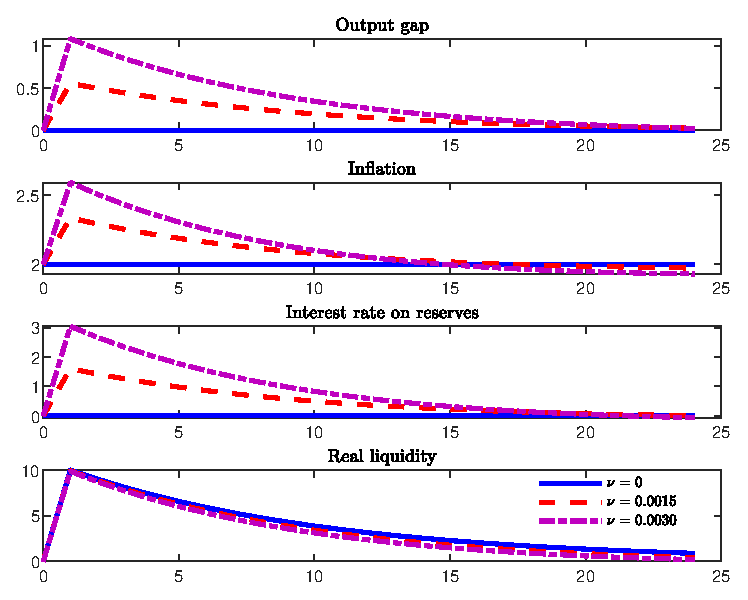
\includegraphics[width=\linewidth]{Figure13}
\caption{Impulse Response to a Shock in the Overall Liquidity Supply}
\label{Figure8.2}
\end{figure}
\end{column}

% -------- Right column: description --------
\begin{column}{0.5\textwidth}
\small
\begin{itemize}
\item Nominal government debt in deviations from the steady state follows the process $\hat{B}_t^{g} = \rho_b \hat{B}_{t-1}^{g} + \varepsilon_{2,t}$
with $0 \le \rho_b \le 1$. 
\vspace{1em}

\item In equilibrium $\hat{B}_t^{g}=\rho\hat{d}_t$.

\vspace{1em}
\item The Figure shows the responses of output gap, inflation, interest rate on reserves, real liquidity to a one-time shock $\varepsilon_{2,t}$.
\end{itemize}
\end{column}
\end{columns}
\end{frame}

%-----------------------------------------------------------
\begin{frame}{Impulse Response to a Liquidity Shock} 

\begin{itemize}
  \item With $\nu>0$, liquidity directly affects aggregate demand:
  \begin{itemize}
    \item Higher liquidity raises the output gap through the AD equation,
    \item This translates into higher inflation.
  \end{itemize}
\vspace{1em}
  \item Monetary and fiscal policies affect the economy not only through interest rates:
 
 \begin{itemize}
    \item Government debt and central bank reserves influence economic activity,
    \item They complement conventional interest-rate policy.
  \end{itemize}
\vspace{1em}
  \item Expanding government liquidity boosts demand:
  \begin{itemize}
    \item Higher government liquidity raises deposits, lowers the liquidity premia and the credit-market interest rate, and pushes consumption and output up,
    \item Increased economic activity feeds into inflation via the AS equation \eqref{8.20}.
  \end{itemize}
\end{itemize}

\end{frame}

%===========================================================
\section{Optimal policy}

%-----------------------------------------------------------
\begin{frame}{Optimal Liquidity Policy}
\small
\begin{itemize}
  \item Optimal policy maximizes household welfare, which now includes utility from holding real deposits.
  \vspace{0.4em}

  \item With lump-sum taxes, optimal policy \textbf{satiates liquidity}:
  \[
    V_d(\cdot)=0,
  \]
  eliminating liquidity premia in equilibrium.
  \vspace{0.4em}

  \item \textcite{friedman1960program} logic:
  \begin{itemize}
    \item The optimal allocation closes the wedge between money-market rates and the policy rate.
    \item When liquidity is interest-bearing, full satiation does \textbf{not} restrict the choice of the inflation target (unlike in Chapter~2).
  \end{itemize}
  \vspace{0.4em}

  \item With distortionary taxes, full liquidity satiation is no longer optimal:
  \begin{itemize}
    \item A second-best trade-off arises between liquidity provision and tax distortions.
  \end{itemize}
\end{itemize}
\end{frame}

%-----------------------------------------------------------
\begin{frame}{Optimal Policy with Lump-Sum Taxes}

\begin{itemize}
    \item We focus on optimal stabilization when lump-sum taxes are available and the steady-state subsidy $\tau_t^s$ offsets monopolistic distortions.
\vspace{1em}
  \item Liquidity assumptions near satiation:
  \begin{itemize}
    \item The economy is close to first-best liquidity satiation ($V_d$ small, $\nu$ small).
    \vspace{0.5em}
    \item Liquidity demand remains well defined below the satiation level.
    \vspace{0.5em}
    \item In the limit, deposit demand retains the form of \eqref{8.23} with $d_y = 0$ and $d_i = -U_c/(V_{dd}d)$.
  \end{itemize}
\end{itemize}

\end{frame}

\begin{frame}[label=Loss Function]{Quadratic Loss Function with Liquidity}

\begin{itemize}
  \item Under the assumptions stated above, the second-order approximation of household utility implies the loss function:
\end{itemize}

\begin{align}
  E_{t_0}\!\left\{
  \sum_{t=t_0}^{\infty} \beta^{t-t_0}
  \left[
    \frac{1}{2}(\hat Y_t - \hat Y_t^e)^2
    + \frac{1}{2}\Lambda_d(\hat d_t - d^*)^2
    + \frac{1}{2}\frac{\theta}{\kappa}(\pi_t - \pi)^2
  \right]
  \right\}. \label{8.27}
\end{align}

\begin{itemize}
  \item The policymaker trades off stabilization of the output gap $(\hat Y_t - \hat Y_t^e)$, inflation deviations $(\pi_t - \pi)$ and real liquidity deviations $(\hat d_t - d^*)$.

  \item The liquidity target $d^* = \nu d_i$ captures steady-state liquidity distortions and is of the same order as the liquidity parameter $\nu$.
 \item In the first best case, liquidity is fully satiated and $\hat d_t = d^*$.
 \vspace{0.1cm}
\begin{center}
\hyperlink{Appendix H.1}{\beamerbutton{Derivation of Quadratic Loss Function with Liquidity (Appendix)}}
\end{center}
\end{itemize}

\end{frame}

\begin{frame}{Optimal Stabilization Policy}

\begin{itemize}
  \item The policymaker minimizes the quadratic loss function subject to the
  \textbf{AS equation}:
  \begin{align}
    \pi_t - \pi
    = \kappa(\hat Y_t - \hat Y_t^e)
      + \upsilon_t
      + \beta E_t(\pi_{t+1} - \pi), \label{8.28}
  \end{align}
  where
  \[
    \upsilon_t = \frac{\kappa}{\sigma^{-1}+\eta}\,\hat\mu_t,
    \qquad
    \hat Y_t^e = \frac{1+\eta}{\sigma^{-1}+\eta}\,\hat A_t .
  \]

  \item The minimization problem is also subject to the \textbf{AD equation}.
  When $\nu$ is of a small order:
  \begin{itemize}
    \item Equilibrium in the liquidity market remains of the same form as in
    \eqref{8.23}, with $d_y = 0$ and $d_i = -\frac{U_c}{V_{dd} d}$.
    \item The functional form of the AD equation \eqref{8.21} is unchanged while $\nu = 0$ in \eqref{8.22}.
  \end{itemize}
\end{itemize}

\end{frame}

\begin{frame}{Optimal Liquidity and Stabilization Policy}
\small
\begin{itemize}
  \item In the limit $\nu \to 0$, the aggregate demand equation \eqref{8.25} becomes:
  \begin{align}
    \hat Y_t
    = E_t \hat Y_{t+1}
      - \sigma\!\left(
        \hat{\imath}_t^X - E_t(\pi_{t+1}-\pi)
        + E_t\Delta\hat\xi_{t+1}
      \right)
      + \rho^{-1} d_i^{-1}\sigma\,\hat d_t. \label{8.29}
  \end{align}
  \vspace{0.4em}

  \item \textbf{Optimal liquidity policy:}
  liquidity is fully satiated, so that
  \[
    d_t = d^* \quad \text{at all times}.
  \]
  \vspace{0.4em}

  \item With liquidity optimally set, the remaining policy problem coincides
  with the standard NK stabilization problem.
\end{itemize}
\end{frame}

\begin{frame}{Optimal Policy and Liquidity}
\small
\begin{itemize}
  \item Combining the targeting rule with the AS equation \eqref{8.28} yields
  the \textbf{same optimal response to shocks} as in Chapter~7.
  \vspace{0.4em}

  \item The key reason is that liquidity is an \textbf{additional policy instrument}:
  under optimal policy it is always set to its efficient level,
  \[
    d_t = d^*,
  \]
  closing liquidity premia.
  \vspace{0.4em}

  \item As a result:
  \begin{itemize}
    \item The steady-state spread between money-market rates and the policy rate is eliminated.
    \item All risk-free rates move together, as implied by the AD equation \eqref{8.29}.
  \end{itemize}
  \vspace{0.4em}

  \item In the absence of markup shocks, the \textbf{first best} is attainable:
  output, inflation, and liquidity deviations can be simultaneously stabilized
  in the loss function \eqref{8.27}.
\end{itemize}
\end{frame}

\begin{frame}{Broader Implications}
\small
\begin{itemize}
  \item In the presence of markup shocks, a trade-off between output and inflation stabilization emerges,
  but it remains optimal to \textbf{fully satiate liquidity} and eliminate money-market spreads.
  \vspace{0.3em}

  \item Liquidity frictions therefore matter primarily when policy is \textbf{sub-optimal},
  as illustrated by the responses in Figure~\ref{Figure8.2}.
  \vspace{0.3em}

  \item From a normative perspective, the policymaker uses government liquidity
  to operate \textbf{as close as possible to the benchmark NK allocation},
  neutralizing financial frictions whenever feasible.
  \vspace{0.3em}

  \item Chapter~9 introduces an additional friction—\textbf{distortionary taxation}—
  which limits optimal liquidity provision and fundamentally alters the nature
  of stabilization policy.
\end{itemize}
\end{frame}

\section{Main Takeaways}
% Summary
% --- FINAL SLIDE: Main Takeaways ---
\begin{frame}{Main Takeaways}
\small

\begin{itemize}
  \item \textbf{Banking and interest rates:} introducing a banking sector generates a \textbf{hierarchy of risk-free rates}; liquidity premia drive wedges between the policy rate, deposit rate, and credit-market rate.

  \item \textbf{Government liquidity:} reserves and treasury bills affect \textbf{aggregate demand} by influencing liquidity premia, acting as a transmission channel beyond the standard interest-rate channel.

  \item \textbf{Liquidity satiation:} when liquidity is fully satiated, the model collapses to the \textbf{benchmark New Keynesian framework} and monetary policy operates solely through the policy rate.

  \item \textbf{Optimal policy:} under lump-sum taxes, liquidity is optimally satiated at all times; the \textbf{optimal stabilization policy} coincides with standard results of the benchmark NK framework.

  \item \textbf{Frictions and distortions:} liquidity frictions matter primarily under sub-optimal policies or \textbf{distortionary taxation}, which constrain the government's ability to provide optimal liquidity.
\end{itemize}

\end{frame}


\section{Bibliography}

\begin{frame}{References}
\printbibliography
\end{frame}

%===========================================================
\appendix
\section{Appendix}
%===========================================================

%-----------------------------------------------------------
\begin{frame}[label=Appendix H]{Appendix: steady state}
\small
\begin{itemize}
  \item Deterministic steady state with constant shocks:
  \[
    \xi_t = \xi,\qquad A_t = A,\qquad \mu_t = 1.
  \]
  \item Markup distortion eliminated by subsidy:
  \[
    \tau^s=\frac{1}{\theta-1}.
  \]
  \item Inflation at target: $\Pi_t=\Pi$.
  \item AS block \eqref{8.14}--\eqref{8.16} implies:
  \[
    F=J,\qquad
    F=\frac{\xi U_c(Y)Y}{1-\alpha\beta},\qquad
    J=\frac{\xi(Y/A)^{1+\eta}}{1-\alpha\beta}.
  \]
  \item Efficient steady-state output:
  \[
    \left(\frac{Y}{A}\right)^\eta = AY\,U_c(Y).
  \]
\end{itemize}
\end{frame}

%-----------------------------------------------------------
\begin{frame}{Appendix: steady state}
\begin{itemize}
  \item Euler equation \eqref{8.13} with $\Pi_t=\Pi$:
  \[
    1+i=\beta^{-1}\Pi.
  \]
  \item Assume $D/P<\bar d$ and collateral binds: $B^g=\rho D$.
  \item Define $\nu\equiv V_d/U_c$ in steady state. Then:
  \[
    1+i^D=(1-\nu)(1+i). \tag{\ref{8.19.5}}
  \]
  \[
    1+i^D=\rho(1+i^X)+(1-\rho)(1+i). \tag{\ref{8.19.75}}
  \]
  \item Combining:
  \[
    \frac{1+i}{1+i^X}=\frac{\rho}{\rho-\nu},\qquad
    \frac{1+i^D}{1+i^X}=\frac{\rho(1-\nu)}{\rho-\nu},
    \qquad (\nu<\rho)\Rightarrow i>i^D>i^X.
  \]
\end{itemize}
\end{frame}

%-----------------------------------------------------------
\begin{frame}{Appendix: derivation of the log-linear approximation}
\begin{itemize}
  \item Start from \eqref{8.11} and subtract steady state:
  \[
    i_t^D - i^D = \rho(i_t^X - i^X) + (1-\rho)(i_t - i).
  \]
  \item Divide by $(1+i^D)$ and use first-order log deviations:
  \[
    \hat\imath_t^D
    = \rho\frac{1+i^X}{1+i^D}\hat\imath_t^X
      + (1-\rho)\frac{1+i}{1+i^D}\hat\imath_t. \tag{\ref{H.2}}
  \]
  \item Using steady-state ratios (via $\nu$) implies:
  \[
    \hat\imath_t^D
    = \frac{\rho-\nu}{1-\nu}\hat\imath_t^X
      + \frac{1-\rho}{1-\nu}\hat\imath_t
    \;\Rightarrow\;
    \hat\imath_t
    = \hat\imath_t^X
      + \frac{1-\nu}{\rho-\nu}(\hat\imath_t-\hat\imath_t^D). \tag{\ref{8.22}}
  \]
\end{itemize}
\end{frame}

%-----------------------------------------------------------
\begin{frame}{Appendix: deposit demand}
\begin{itemize}
  \item First-order approximation of \eqref{8.12} implies:
  \[
    (1-\nu)(\hat\imath_t^D-\hat\imath_t)
    =
    -\frac{V_{dd}d}{V_d}\nu\,\hat d_t
    -\frac{U_{cc}Y}{U_c}\nu\,\hat Y_t.
  \]
  \item Using $\sigma_d\equiv -\frac{V_d}{V_{dd}d}$ and $\sigma\equiv -\frac{U_{cc}Y}{U_c}$:
  \[
    \hat d_t
    = d_y\hat Y_t
      - d_i(\hat\imath_t-\hat\imath_t^D),
    \qquad
    d_y=\frac{\sigma_d}{\sigma},\quad
    d_i=\sigma_d\frac{1-\nu}{\nu}. \tag{\ref{8.23}}
  \]
\end{itemize}
\end{frame}

%-----------------------------------------------------------
\begin{frame}{Appendix: AD equation, forward solution}
\begin{itemize}
  \item Solving \eqref{8.25} forward:
  \begin{align}
    \hat Y_t
    &=
    -\nu_\rho\sigma
    E_t\sum_{T=t}^{\infty}
    \nu_\rho^{\,T-t}
    \Big(
      \hat\imath_T^X
      -(\pi_{T+1}-\pi)
      +\Delta\hat\xi_{T+1}
    \Big)
    \nonumber\\
    &\quad
    +d_y^{-1}(1-\nu_\rho)
    E_t\sum_{T=t}^{\infty}
    \nu_\rho^{\,T-t}\hat d_T.
    \label{8.26}
  \end{align}
  \item $\nu_\rho<1$ implies geometrically decaying weights on future policy and future liquidity.
\end{itemize}
\vspace{0.1cm}
\begin{center}
\hyperlink{Rate Mapping}{\beamerbutton{Back to Log-Linear Rate Mapping}}
\end{center}
\end{frame}

%-----------------------------------------------------------
\begin{frame}[label=Appendix H.1]{Appendix: Loss Function Derivation}

\begin{itemize}
  \item The loss function \eqref{8.27} is obtained as a second-order approximation of household utility \eqref{8.7}, following Chapter~7.
  \item We focus on the liquidity term $V(d_t)$, assuming:
  \begin{itemize}
    \item The economy is close to liquidity satiation: $V_d = \mathcal{O}(\|\xi\|)$,
    \item The liquidity parameter $\nu$ is of small order.
  \end{itemize}
  \item As $d_t$ approaches the satiation level $\bar d$ from below:
  \begin{itemize}
    \item $V_{dd}<0$, ensuring a well-defined liquidity demand.
    \item In the limit $V_d \to 0$, liquidity demand retains the form of \eqref{8.23} with
    \[
      d_y = 0,
      \qquad
      d_i = -\frac{U_c}{V_{dd}d}.
    \]
  \end{itemize}
\end{itemize}

\end{frame}


%-----------------------------------------------------------
\begin{frame}{Appendix: Loss Function Derivation}

Consider a second-order Taylor expansion of $V(d_t)$:
\begin{align*}
V(d_t)
&= V(d)
  + V_d(d_t-d)
  + \tfrac12 V_{dd}(d_t-d)^2
  + \mathcal{O}(\|\xi\|^3).
\end{align*}

Using
\[
(d_t-d)=d\!\left(\hat d_t + \tfrac12 \hat d_t^2\right)
  + \mathcal{O}(\|\xi\|^3),
\]
we obtain:
\begin{align*}
V(d_t)
&= V(d)
 + V_d d\,\hat d_t
 + \tfrac12 (V_d d + V_{dd} d^2)\hat d_t^2
 + \mathcal{O}(\|\xi\|^3).
\end{align*}

Neglecting terms independent of policy:
\begin{align*}
V(d_t)
&= U_c Y
\left[
\frac{V_d d}{U_c Y}\hat d_t
+ \tfrac12\frac{V_{dd} d^2}{U_c Y}\hat d_t^2
\right]
+ \mathcal{O}(\|\xi\|^3).
\end{align*}

\end{frame}

%-----------------------------------------------------------
\begin{frame}{Appendix: Loss Function Derivation}

Using
\[
\nu \equiv \frac{V_d}{U_c},
\qquad
d_i \equiv -\frac{U_c}{V_{dd} d},
\]
we can write:
\begin{align*}
V(d_t)
&= U_c Y\,\frac{d}{Y}
\left[
\nu \hat d_t
- \tfrac12 \frac{1}{d_i}\hat d_t^2
\right]
+ \mathcal{O}(\|\xi\|^3).
\end{align*}

Conclude that:
\begin{align*}
V(d_t)
&=
-\tfrac12 \frac{U_c d}{d_i}
\big(\hat d_t - d^*\big)^2
+ \mathcal{O}(\|\xi\|^3),
\end{align*}
where $d^* \equiv \nu d_i$.
\end{frame}

\begin{frame}{Appendix: Loss Function Derivation}

\begin{itemize}
  \item Result from chapter ~7 (utility approximation):
  \begin{align*}
    U_{t_0}
    = -(\sigma^{-1}+\eta)L^{1+\eta}
    E_{t_0}\sum_{t=t_0}^{\infty}\beta^{t-t_0}
    \left[
      \frac{1}{2}(\hat Y_t - \hat Y_t^e)^2
      + \frac{\theta}{2\kappa}(\pi_t - \pi)^2
    \right]
    + \text{t.i.p.}
  \end{align*}
    \item Combining this expression with the previously derived liquidity term and defining $\Delta \equiv \frac{d}{Y d_i}$ yields the quadratic loss function \eqref{8.27}:
  \begin{align*}
    E_{t_0}\sum_{t=t_0}^{\infty}\beta^{t-t_0}
    \left[
      \frac{1}{2}(\hat Y_t - \hat Y_t^e)^2
      + \frac{1}{2}\Delta(\hat d_t - d^*)^2
      + \frac{\theta}{2\kappa}(\pi_t - \pi)^2
    \right],
  \end{align*}
  which corresponds to equation~\eqref{8.27}.
\end{itemize}
\vspace{0.1cm}
\begin{center}
\hyperlink{Loss Function}{\beamerbutton{Back to Loss Function}}
\end{center}
\end{frame}




\end{document}